\documentclass[tikz]{standalone}
\usepackage{graphicx} % Required for inserting images
\usepackage{tikz}
\usetikzlibrary{shadows}
\usepackage{xcolor}
\usetikzlibrary{backgrounds}
\usetikzlibrary {shapes.geometric,shapes.misc}

\usetikzlibrary {arrows.meta,automata,positioning,fit,calc}

\definecolor{ProcessStepBackground}{HTML}{FFFAF0}
\definecolor{IntermediateStateColour}{HTML}{949698}

\tikzstyle{SinkLevel} =[draw,trapezium,trapezium stretches body,trapezium left angle=100, trapezium right angle=100,rotate=180]
\tikzstyle{Storagelevel}=[draw,chamfered rectangle,chamfered rectangle xsep=2cm ]
\tikzstyle{SourceLevel} =[draw,trapezium,trapezium stretches body,trapezium left angle=100, trapezium right angle=100,]
\tikzstyle{NetworkLevelCore} =[inner sep=0.25cm]
% \tikzstyle{NetworkLevelCore} =[draw,trapezium,trapezium stretches body,trapezium left angle=100, trapezium right angle=100]
\tikzstyle{InfinitesimalNode}=[circle,draw=none,inner sep=0pt,minimum size=0pt]
\tikzstyle{ProcessStepNode} =[draw,fill=ProcessStepBackground,rounded corners,text width=2 cm,align=center]
\tikzstyle{IdleState} =[fill=yellow,rounded corners]
\tikzstyle{OutputState} =[fill=red,rounded corners]
\tikzstyle{InputState} =[fill=green,rounded corners]
\tikzstyle{IntermediateState} =[fill=IntermediateStateColour,rounded corners]
\tikzstyle{Source} =[fill=ProcessStepBackground,shape border rotate=90,aspect=0.1,draw]
\tikzstyle{Sink} =[fill=ProcessStepBackground,shape border rotate=90,aspect=0.1,draw]
\tikzstyle{SourceOrSink} =[fill=ProcessStepBackground,cylinder, shape border rotate=90,aspect=0.1,draw,text width=2 cm,align=center]
\tikzset{
diagonal fill/.style 2 args={fill=#2, path picture={
\fill[#1, sharp corners] (path picture bounding box.south west) -|
                         (path picture bounding box.north east) -- cycle;}},
reversed diagonal fill/.style 2 args={fill=#2, path picture={
\fill[#1, sharp corners] (path picture bounding box.north west) |- 
                         (path picture bounding box.south east) -- cycle;}}
}


\newcommand{\CreateStorageHexagon}[2]{
\draw[-] let \p{left_upper_point}=(#1.south west),
    \p{right_upper_point}=(#1.south east),
    \p{left_lower_point}=(#2.north west),
    \p{right_lower_point}=(#2.north east),
    \n{vertical_distance}={(\y{left_upper_point}-\y{left_lower_point})},
    \p{right_point}=(\x{right_upper_point}+0.5cm,\y{right_upper_point}-\n{vertical_distance}/2),
    \p{left_point}=(\x{left_upper_point}-0.5cm,\y{left_upper_point}-\n{vertical_distance}/2),
    in (\p{left_upper_point}) ->(\p{left_point}) -> (\p{left_lower_point})->(\p{right_lower_point})->(\p{right_point})->(\p{right_upper_point})--(\p{left_upper_point});}

\newcommand{\CreateSinkTrapezium}[2]{
    \draw[-] let \p{left_upper_point}=(#1.south west),
        \p{right_upper_point}=(#1.south east),
        \p{sink_middle_point}=(#2),
        \n{vertical_distance}={(\y{left_upper_point}-\y{sink_middle_point})},
        % \n{y_shift_outer}=1cm,
        \p{left_point}=(\x{left_upper_point}-0.5cm,\y{sink_middle_point}-\n{vertical_distance}),
        \p{right_point}=(\x{right_upper_point}+0.5cm,\y{sink_middle_point}-\n{vertical_distance}),
        in (\p{left_upper_point}) -- (\p{left_point}) -- (\p{right_point})--(\p{right_upper_point}) --(\p{left_upper_point});}

\newcommand{\CreateSourceTrapezium}[2]{
    \draw[-] let \p{left_lower_point}=(#1.north west),
        \p{right_lower_point}=(#1.north east),
        \p{source_middle_point}=(#2),
        \n{vertical_distance}={(\y{source_middle_point}-\y{left_lower_point})},
        % \n{y_shift_outer}=1cm,
        \p{left_upper_point}=(\x{left_lower_point}-0.5cm,\y{source_middle_point}+\n{vertical_distance}),
        \p{right_upper_point}=(\x{right_lower_point}+0.5cm,\y{source_middle_point}+\n{vertical_distance}),
        in  (\p{left_lower_point}) --(\p{left_upper_point}) -- (\p{right_upper_point})--(\p{right_lower_point}) -- (\p{left_lower_point});}


\tikzstyle{InputAndOutputState} =[diagonal fill={red}{green},rounded corners, drop shadow,draw ]

\begin{document}
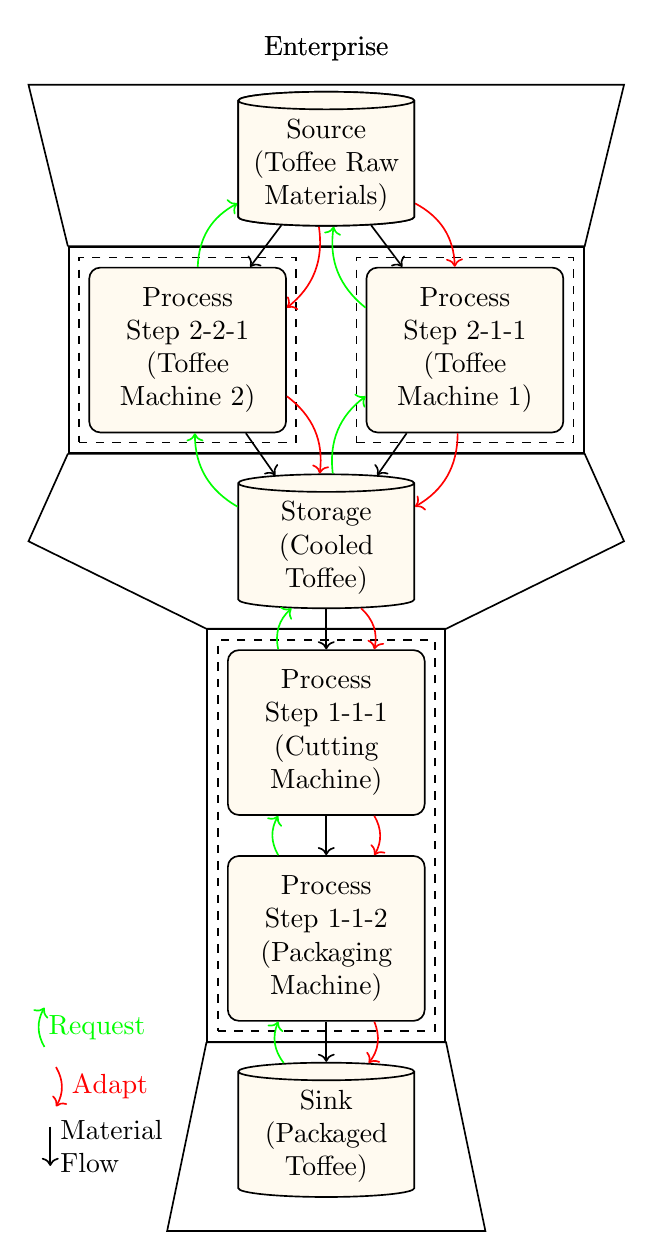
\begin{tikzpicture}[->,auto,node distance=0.25cm,on grid,semithick]
    \node[SourceOrSink](Packaged-Toffee-Sink){Sink \\(Packaged Toffee)};

    \matrix [column sep=0.5cm,row sep=0.5cm,draw, nodes={rectangle, anchor=center},NetworkLevelCore,above= of Packaged-Toffee-Sink.north](6dd744d7-4069-4272-8eaf-f1879d1860a1){
        \node[ProcessStepNode](Cutting-Machine){Process Step 1-1-1\\ (Cutting Machine)};     \\
        \node[ProcessStepNode](Packaging-Machine){Process Step 1-1-2\\ (Packaging Machine)}; \\
    };

    \node[fit=(Cutting-Machine)(Packaging-Machine),dashed,draw]{};
    \CreateSinkTrapezium{6dd744d7-4069-4272-8eaf-f1879d1860a1}{Packaged-Toffee-Sink}

    % \node[,SinkLevel,minimum height=2cm]at (0,3){} ;
    \node[SourceOrSink,above= of 6dd744d7-4069-4272-8eaf-f1879d1860a1.north](Cooled-Toffee-Storage){Storage (Cooled Toffee)};

    \matrix [column sep=1cm,row sep=0.5cm,draw, nodes={rectangle, anchor=center},NetworkLevelCore,above= of Cooled-Toffee-Storage.north](b2da0516-bcb6-4dc9-946f-a442e4d4797f){
        \node[ProcessStepNode](Toffee-Machine-2){Process Step 2-2-1\\ (Toffee Machine 2)}; &
        \node[ProcessStepNode](Toffee-Machine-1){Process Step 2-1-1\\ (Toffee Machine 1)};   \\
    };
    \node[fit=(Toffee-Machine-2),dashed,draw]{};
    \node[fit=(Toffee-Machine-1),dashed,draw]{};

    \CreateStorageHexagon{b2da0516-bcb6-4dc9-946f-a442e4d4797f}{6dd744d7-4069-4272-8eaf-f1879d1860a1}
    \node[SourceOrSink,above= of b2da0516-bcb6-4dc9-946f-a442e4d4797f.north](Toffee-Raw-Materials){Source (Toffee Raw Materials)};
    \node[,above= of Toffee-Raw-Materials.north](TitleNode){Enterprise};

    \node[left= of Packaged-Toffee-Sink.west,xshift=-2cm,yshift=-0.5cm](down_node){};
    \node[above= 0.5 cm of down_node.north](upward_node_node){};
    \node[above= 0.5 cm of upward_node_node.north](upward_node_node1){};
    \node[above= 0.5 cm of upward_node_node1.north](upward_node_node2){};
    \CreateSourceTrapezium{b2da0516-bcb6-4dc9-946f-a442e4d4797f}{Toffee-Raw-Materials};
    \path[<-] (upward_node_node) edge[bend right=30,red] node[right]{Adapt}(upward_node_node1);
    \path[->] (upward_node_node) edge[] node[right,align=left]{Material\\ Flow}(down_node);
    \path[->] (upward_node_node1) edge[bend left=30,green] node[right]{Request}(upward_node_node2);

    \path[<-] (Cooled-Toffee-Storage) edge[bend right=30,green] (Cutting-Machine);
    \path[->] (Cooled-Toffee-Storage) edge[bend left=30,red] (Cutting-Machine);
    \path[<-] (Cutting-Machine) edge[bend right=30,green] (Packaging-Machine);
    \path[->] (Cutting-Machine) edge[bend left=30,red] (Packaging-Machine);
    \path[<-] (Packaging-Machine) edge[bend right=30,green] (Packaged-Toffee-Sink);
    \path[->] (Packaging-Machine) edge[bend left=30,red] (Packaged-Toffee-Sink);

    \path[<-] (Toffee-Raw-Materials) edge[bend right=30,green] (Toffee-Machine-2);
    \path[->] (Toffee-Raw-Materials) edge[bend left=30,red] (Toffee-Machine-2);
    \path[<-] (Toffee-Machine-2) edge[bend right=30,green] (Cooled-Toffee-Storage);
    \path[->] (Toffee-Machine-2) edge[bend left=30,red] (Cooled-Toffee-Storage);

    \path[<-] (Toffee-Raw-Materials) edge[bend right=30,green] (Toffee-Machine-1);
    \path[->] (Toffee-Raw-Materials) edge[bend left=30,red] (Toffee-Machine-1);
    \path[->] (Toffee-Machine-1) edge[bend left=30,red] (Cooled-Toffee-Storage);
    \path[<-] (Toffee-Machine-1) edge[bend right=30,green] (Cooled-Toffee-Storage);


    \node[SourceOrSink,above= of b2da0516-bcb6-4dc9-946f-a442e4d4797f.north](Toffee-Raw-Materials){Source (Toffee Raw Materials)};
    \node[,above= of Toffee-Raw-Materials.north](TitleNode){Enterprise};
    \draw[] (Cooled-Toffee-Storage) -> (Cutting-Machine);
    \draw[] (Cutting-Machine) -> (Packaging-Machine);
    \draw[] (Packaging-Machine) -> (Packaged-Toffee-Sink);
    \draw[] (Toffee-Raw-Materials) -> (Toffee-Machine-2);
    \draw[] (Toffee-Machine-2) -> (Cooled-Toffee-Storage);
    \draw[] (Toffee-Raw-Materials) -> (Toffee-Machine-1);
    \draw[] (Toffee-Machine-1) -> (Cooled-Toffee-Storage);


    % \path[->,draw] (ProcessStep1Control) edge[bend right=30,green] node{Request}(SourceControl);
\end{tikzpicture}
\end{document}
